\chapter{Ecoulements visqueux}
\label{ch:newtonien}

\section{Equation de Navier-Stokes pour fluide Newtonien, incompressible}

Dans le chapitre~\ref{ch:euler}, nous avons établi l'équation d'Euler pour un fluide parfait, en négligeant les effets de la viscosité. Cependant, dans la réalité, les fluides réels (comme l'eau ou l'air) présentent une résistance interne au mouvement, due aux frottements entre couches de fluide. 

\begin{figure}
  \begin{center}
    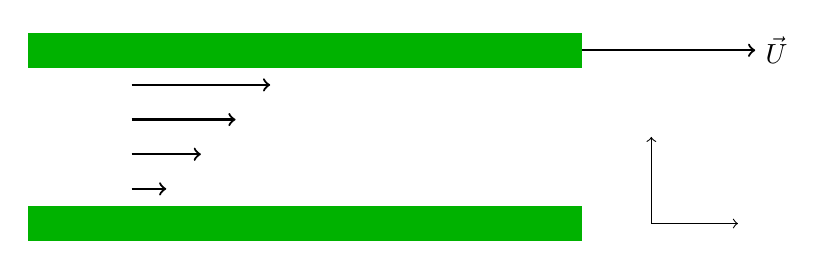
\begin{tikzpicture}[scale=2.2] % adjust scale so total width ≈ 6 cm
  \tikzset{plate/.style={fill=green!70!black, draw=none}}
  
  % Lower plate: from (-0.6,-0.1) to (2.6,0.1)
  \draw[plate] (-0.6,-0.1) rectangle (2.6,0.1);
  
  % Upper plate: from (-0.6,0.9) to (2.6,1.1)
  \draw[plate] (-0.6,0.9) rectangle (2.6,1.1);

  % Flow arrows at y = 0.2,0.4,0.6,0.8
  \draw[->, thick] (0,0.2) -- (0.2,0.2);
  \draw[->, thick] (0,0.4) -- (0.4,0.4);
  \draw[->, thick] (0,0.6) -- (0.6,0.6);
  \draw[->, thick] (0,0.8) -- (0.8,0.8);

  \draw[->] (3.,0) -- (3.5,0) node[right] {$\ex$};
  \draw[->] (3.,0) -- (3.0,0.5) node[above] {$\ez$};
  % Velocity arrow on the right side of the upper plate
  % Length approx = 1.0
  \draw[->, thick] (2.6,1.0) -- ++(1.0,0) node[right] {$\vec{U}$};
\end{tikzpicture}


  \end{center}
  \caption{Expérience idéalisée représentant la viscosité d'un fluide entre deux plaques présentant entre elles un différentiel de vitesse  $U$ sur une épaisseur $h$. La force par unité de surface ($A$) à exercer sur la plaque supérieure en régime stationnaire est $\od{\vec{F}}{A}= \mu U/h$}\label{fig:couette}
\end{figure}

On aborde la notion de viscosité dans le régime laminaire par l'expérience de l'écoulement de Couette. Soit une couche de fluide prise entre deux plaques présentant entre elles une différence de vitesse $\vec{U}$. Si le fluide est suffisament visqueux, la couche suffisament fine, et la vitesse suffisament petite (ce sont des éléments que nous allons préciser), la vitesse du fluide adopte un profil linéaire, sans glissement par rapport aux deux parois mobiles, et la force par unité d'aire ($A$) à exercer sur la plaque supérieure pour conserver un régime stationnaire  est $\od{\vec{F}}{A}=\mu \vec{U}/h$, ce qui est équivalent à affirmer que la force par unité d'aire exercée par le fluide sur cette plaque est $-\od{\vec{F}}{A}$. 

Cette force par unité de surface porte le nom de contrainte, et il s'agit plus particulièrement ici d'une \cindex{contrainte tangentielle}, notée $\tau_{zx}$:


\begin{displaymath}
  \tau_{zx} = \mu U/h
\end{displaymath}

Le second indice, $x$, fait référence à la direction de la force (par unité de surface). Le premier indice,  $z$, fait référence s'exerce sur la face supérieure du fluide, dont la nomale est dirigée dans la direction de l'aexe $\ez$. Nous verrons dans peu de temps que $\tau_{zx}$ est la composante d'un \cindex{tenseur des contraintes}. 

\todo{dans le schéma, utiliser la notation $\tau$}

L'expérience est idéalisée à beaucoup d'égards et il ne faut pas se laisser distraire par les intéractions spécifiques entre le fluide et la plaque. Le point important est que le fluide présente une \emph{résistance au cisaillement}. Nous pouvons formaliser le phénomène à l'échelle d'un élement fluide. Considérons trois éléments, empilé selon l'axe $\ez$, caractérisés par une vitesse horizontale $U(z)$. A l'échelle de ce volume élémentaire, l'expression linéaire adoptée pour l'écoulement de Couette suggère que le bloc supérieur exerce une force de composante horizontale  $\dif F_x = -\mu \od{U}{z}(z+\frac{1}{2}\dif z)\dif x\dif y$ sur le bloc intermédiaire, et le bloc inférieur exerce une force de composante horizontale $\dif F_x = \mu \od{U}{z}(z-\frac{1}{2}\dif z)\dif x\dif y$. 

On peut donc modéliser la somme des forces de viscosité, par unité de volume, dans cet écoulement laminaire $U(z)$ par 

\begin{equation}
  \dif F_x = \od{}{z} \mu \od{U}{z} \dif V =  \mu \od[2]{U}{z} \dif V. 
  \label{eq:newtonnien}
\end{equation}

On est donc tenté de compléter le raisonnement qui a a abouti à l'équatieur d'Euler \eqref{eq:euler} pour y intégrer ce phénomène de viscosité. Considérons d'abord exclusivement l'effet d'un cisaillement selon $\ez$, sur la composante $\ex$ de la vitesse:

\begin{displaymath}
  \rho \, \Dt{u_x} = - \rho \, \grad \gpot - \grad p + \mu \od[2]{u_x}{z} 
\end{displaymath}

Par symmétrie, un cisaillement selon $\ey$ aura le même effet, qui doit donc être ajouté à la même équation

\begin{displaymath}
  \rho \, \Dt{u_x} = - \rho \, \grad \gpot - \grad p + \mu ( \od[2]{u_x}{x} + \od[2]{u_x}{y} )
\end{displaymath}

Avec un peu d'audace, nous pourrions suggérer qu'un différentiel de vitessse selon l'axe $\ex$ génère une force que l'on peut paramétriser de la même manière (résistance à l'étirement):

\begin{equation}
  \rho \, \Dt{u_x} = - \rho \, \grad \gpot - \grad p + \mu ( \od[2]{u_x}{x} + \od[2]{u_x}{y} +  \od[2]{u_x}{z} )
  \label{eq:diffusion_ux}
\end{equation}

On peut justifier notre audace en reconnaissant, dans l'équation \eqref{eq:diffusion_ux} un analogue à l'équation de la chaleur. De la même façon que l'énergie se diffuse par l'effet cumulé des chocs moléculaires, la quantité de mouvement de \emph{diffuse}, également par échange lors des collisions. L'analogie est très imparfaite car en réalité les forces d'attraction jouent un rôle majeur dans le phénomène de diffusion. Nous allons donc admettre cette équation. Elle est bien correcte. C'est l'équation de Navier-Stokes pour un fluide newtonien incompressible, mais elle doit être justifiée plus soigneusement. C'est l'objet de la section \ref{sect:ns}. 

\begin{figure}
  \begin{center}
    \begin{tikzpicture}[scale=1.0]

% Styles
\tikzset{
  outer/.style={dotted, draw=black, line width=0.4pt},
  middle/.style={draw=black, line width=1.5pt},
  force/.style={->, thick, blue!70!black},
  vel/.style={->, line width=1pt},
}

% --- Three rectangles ---
% Left block
\draw[outer] (-1,-1) rectangle (2,0);

% Middle block (thick)
\draw[middle] (-0.8,0) rectangle (2.2,1);

% Right block
\draw[outer] (-0.6,1) rectangle (2.4,2);

% --- Axes arrows ---
\draw[->, thick] (-3.2,0) -- (-3.2,1.0) node[midway,left] {$\ez$};
\draw[->, thick] (-3.2,0) -- (-2.2,0) node[midway,below] {$\ex$};

% --- Velocity vectors on middle block ---
% Coordinates of centers of top and bottom faces of middle block
\coordinate (bottomcenter) at (0.7,-0.1);
\coordinate (topcenter)    at (0.7,1.1);
\coordinate (bottomright) at (2.3,0);
\coordinate (topright)    at (2.3,1.0);

% Velocities (black)
\draw[vel] (bottomright) -- ++(0.8,0)
  node[right] {$U\!\left(z-\tfrac12 \,\mathrm dz\right)$};

\draw[vel] (topright) -- ++(1.0,0)
  node[right] {$U\!\left(z+\tfrac12 \,\mathrm dz\right)$};

% Force vectors (dark green)
\draw[force] (bottomcenter) -- ++(0.5,0.0)
node[below] {$\mu\,\frac{\mathrm dU}{\mathrm dz}\!\left(z-\frac{1}{2} \dif z \right)$};

\draw[force] (topcenter) -- ++(-0.5,+0.0)
node[above] {$\mu\,\frac{\mathrm dU}{\mathrm dz}\!\left(z+\frac{1}{2} \dif z\right)$};

% Dots at centers
\fill (bottomright) circle (1.5pt);
\fill (topright) circle (1.5pt);

% --- Dimension markers ---
% Height = dz
\draw[<->] (-1.2,0. ) -- (-1.2,1. )
  node[midway,left] {$\dif z$};

% Length = dx
\draw[<->] (-1.0,-1.3) -- (2.0,-1.3)
  node[midway,below] {$\dif x$};

\end{tikzpicture}




  \end{center}
  \caption{Bilan des forces de viscosité causées par le cisaillement sur un volume élémentaire}
\end{figure}


En trois dimensions, cette équation de Navier-Stokes devient: 

\begin{displaymath}
  \rho \Dt{\u} = -\grad p - \rho \grad \gpot + \mu \lapl \u,
\end{displaymath}
où $\lapl \u = (\lapl u, \lapl v, \lapl w)$ est le \cindex{laplacien} du champ de vitesse, et $\mu$ le \cindex{coefficient de viscosité}. 

Ainsi on a, pour différentes fluides, à 20$^\circ$, 1atm:

\begin{tabular}{|c|c|}
\hline
Fluide & $\mu$ (Pa$\cdot$s) \\
\hline
Air & $1.8 \times 10^{-5}$\\
Hexane & $0.3 10^{-3}$ \\
Eau & $10^{-3}$ \\
Sang &  $4$ à $6\ 10^{-3}$ \\
Huile  d'olive & $0.05$  \\
Miel & $10$ \\
\hline
\end{tabular}

Cette équation sera suffisante pour décrire la plupart des écoulements étudiés dans ce cours, y compris l'\cindex{écoulement de Poiseuille}.





\section{Tenseur des contraintes}

Dans le chapitre~\ref{ch:euler}, nous avons utilisé la \cindex{pression statique} pour décrire les forces normales s'exerçant sur un élément de volume de fluide. Nous avions écrit explicitement :
\begin{displaymath}
  \dif\vec{f} = p \vec{n} \dif A, 
\end{displaymath}
où $\vec{n}$ est un vecteur normal à la surface témoin. Cette expression suppose que la force est purement normale à la surface, ce qui est valable pour un fluide parfait.
Or, nous l'avons vu, la viscosité se manifeste par des forces \emph{tengentielles} à la surface témoin. Ces forces sont proportionnelles à la surface témoin (comme les forces de pressions) mais il nous faut un formalisme mathématique qui permette d'exprimer leur caractère directionnel. C'est l'objet du \cindex{tenseur des contraintes}, $\tensor{\tau}$. La force associée à ce tenseur est maintenant directionnelle (contrairement à sa forme dans \eqref{eq:hydrostat_int} et \eqref{eq:hydrostat_diff}:


\begin{displaymath}
  \dif\vec{f} = \tensor{T} \vec{n} \dif A.
\end{displaymath}

Ce tenseur permet de prendre en compte non seulement les forces normales (pression), mais aussi les forces tangentielles (cisaillement). 

On retrouve le fluide parfait pour  $T_{ij} = -p \delta_{ij}$, que l'on peut écrire synthétiquement sous la forme $\tensor{T} = -p \tensor{1}$, où $\tensor{1}$ est la matrice unitaire. 

On va donc devoir développer et justifier l'existence d'un tenseur $\tensor{\tau}$ qui va venir compléter les effets de pression. L'enjeu est de développer une expression de $\tau$ pour le fluide Newtonien. C'est l'objet de la section suivante. 

\begin{redmargin}

\section{Dérivation formelle de l'équation de Navier-Stokes \label{sect:ns}}

Pour paramétrer $\tensor{\tau}$, nous partons du \cindex{tenseur des déformations} $\tensor{e}$, défini comme la partie symétrique du gradient de vitesse :
\begin{displaymath}
  e_{ij} = \frac{1}{2}\left( \pd{u_i}{x_j} + \pd{u_j}{x_i} \right).
\end{displaymath}
Ce tenseur capture les effets de compression, dilatation et cisaillement du fluide. En supposant que le fluide est newtonien (c'est-à-dire que les contraintes sont proportionnelles aux déformations) et isotrope (les propriétés sont indépendantes de la direction), on montre que le tenseur des contraintes visqueuses s'écrit :
\begin{displaymath}
  \tau_{ij} = 2 \mu e_{ij} + \lambda \delta_{ij} \sum_{m} e_{mm},
\end{displaymath}
où $\mu$ est le coefficient de viscosité dynamique et $\lambda$ le second coefficient de viscosité. La somme $\sum_{m} e_{mm}$ n'est autre que la divergence du champ de vitesse, $\Div \u$.

En combinant ce résultat avec la pression statique, on obtient le tenseur des contraintes total :
\begin{equation}
  T_{ij} = - \left( p + \frac{2}{3} \mu \Div \u \right) \delta_{ij} + 2\mu e_{ij}.
  \label{eq:stress_tensor}
\end{equation}
La trace de ce tenseur, $\sum_i T_{ii}$, donne accès à la pression dynamique $\bar{p}$ :
\begin{displaymath}
  \bar{p} = -\frac{1}{3} \text{Tr}(\tensor{T}) = p + \left( \frac{2}{3}\mu + \lambda \right) \Div \u.
\end{displaymath}
La partie déviatorique du tenseur (de trace nulle) est associée au cisaillement :
\begin{displaymath}
  T_{ij} = - \bar{p} \delta_{ij} + \left( 2 \mu e_{ij} - \frac{2}{3}\mu \Div \u \delta_{ij} \right).
\end{displaymath}
L'\cindex{approximation de Stokes} suppose que $p = \bar{p}$, ce qui implique $\lambda = -\frac{2}{3}\mu$. Dans ce cas, le tenseur des contraintes se simplifie en :
\begin{displaymath}
  T_{ij} = - p \delta_{ij} + \underbrace{2\mu e_{ij} - \frac{2}{3}\mu \Div \u \delta_{ij}}_{\tau_{ij}}, 
\end{displaymath}

que l'on peut réexprimer sous la forme plus synthétique:

\begin{key}{Approximation de Stokes}
\begin{equation}
  \tensor{T} = \tensor{\tau} - \tensor{1}p, \quad\text{avec}\   \tensor{\tau} = 2\mu (\tensor{e} - \frac{1}{3} \Div\u \tensor{1})
  \label{eq:tenseur_contraintes_stokes}
\end{equation}
\end{key}

Pour un fluide incompressible ($\Div \u = 0$), cette expression se réduit à :
\begin{equation}
  \tensor{T} = - \tensor{1}p + 2 \mu \tensor{e}.
  \label{eq:tenseur_contraintes_stokes_incompressible}
\end{equation}


En insérant cette expression dans l'équation du mouvement, on remplace la force de pression par la divergence du tenseur des contraintes :
\begin{equation}
  \rho \, \Dt{\vec{u}} = - \rho \, \grad \gpot + \Div{\tensor{T}}.
  \label{eq:ns}
\end{equation}
La divergence du tenseur $\tensor{T}$ est définie par composante par composante. La composante $i$ répond à
\begin{displaymath}
  (\Div{\tensor{T}})_i = \sum_j \pd{T_{ij}}{x_j}.
\end{displaymath}
En développant ce terme pour un fluide incompressible et en utilisant l'approximation de Stokes, on retrouve (après un peu de calcul) l'équation de Navier-Stokes incompressible :
\begin{equation}
  \rho \Dt{\u} = -\grad p - \rho \grad \gpot + \mu \lapl \u.
  \label{eq:ns_incompressible}
\end{equation}
Cette équation décrit la dynamique des fluides visqueux et sera la base de nos prochains développements, notamment pour l'étude des écoulements laminaires comme celui de Poiseuille.

Par ailleurs, sur base de l'identité:

\begin{displaymath}
\curl(\curl\u) = \grad(\Div{\u}} - \lapl \u
\end{displaymath}

on aura, pour un écoulement incompressible ($\Div\u=0$) une expression équivalente de l'équation \eqref{eq:ns_incompressible}:

\begin{equation}
  \rho \Dt{\u} = -\grad p - \rho \grad \gpot + \mu \curl(\curl \u).
  \label{eq:ns_incompressible_bis}
\end{equation}

\end{redmargin}

\section{Écoulements de Poiseuille}

Nous allons étudier différents types d'écoulement symmétriques. Comme souvent en physique, l'art de résoudre ces écoulement réside dans le choix d'un bon système de coordonnées et l'application judicieuse des conditions aux limites. 

\subsection{Écoulement de Poiseuille plan}

On considère un écoulement stationnaire, où un gradient constant de pression selon $\ex$ contrebalance les forces de viscosité. L'écoulement s'opère entre deux plans infinis. Les plans sont selon les axes $\{\ex, \ey\}$ et l'espace qui sépare les deux plans est selon l'axe $\ez$. 

Par argument de symmétrie, on sait que le seul gradient de pression est selon $\ex$ : $\pd{p}{x} = C$. Par ailleurs,  on admet que si les deux plaques qui bordent le flux sont fixes, $u(z=0) = u(z=h) = 0$ (on parle en Anglais de \emph{\cindex{non-slip boundary conditions}}. On néglige les effets de gravitation. La notation est $\vec{u}=(u,v,w)$. 

S'il n'y a pas de rupture de symmétrie (ce qui est à prouver, nous y reviendrons), la symmétrie des conditions frontière impose $v=w=0$. 

L'équation de Navier-Stokes pour un fluide incompressible \eqref{eq:ns_incompressible} devient, selon l'axe $\ex$: 

\begin{equation}
\rho u \od{u}{x} = -\underbrace{C}_{\od{p}{x}} + \mu \od[2]{u}{x}. 
\label{eq:couette_plan}
\end{equation}

Les dérivées droites remplacent les dérivées partielles car $u$ n'est désormais fonction que d'une seule variable. Nous voyons que le gradient de pression (constant, $C$) est potentiellement équilibré par deux termes: le transport de moment cinétique, dont nous avons vu qu'il agit comme une espèce de force dynamique; et les forces de viscosité. Puisqu'ici nous admettons une symmétrie de translation pour la vitesse (la vitesse est constante selon $\ex$), le membre de gauche s'annule et l'équation se réduit à


\begin{displaymath}
C = \mu \od[2]{u}{x}, 
\end{displaymath}

dont la solution générale est $u = A + Bx + \frac{C}{2\mu}x^2$. Les conditions aux frontières que nous avons choisies imposent la solution

\begin{displaymath}
u(z) = \frac{C}{2\mu} (y^2 - h z).
\end{displaymath}

Le débit volumique, par unité de profondeur (le long de l'axe $\ey$) s'obtient en intégrant la vitesse selon la hauteur $z$:


\begin{displaymath}
  Q = \int_{0}^h u(z)\,\dif z = - \frac{Ch^3}{12\mu}.
\end{displaymath}


\subsection{Écoulement de Poiseuille dans un cylindre}
\label{sec:poiseuille_cylindre}

Nous considérons un problème analogue, mais cette fois en adoptant une conduite cylindrique. Nous admettons toujours un gradient de pression le long de l'horizontale $p=p(x)$, et une vitesse axisymmétrique ($u=u(r)$). Cette fois notre équation devient

\begin{displaymath}
0 = -\od{p}{x} + \frac{\mu}{r} \od{}{r}\left( r \od{u_x}{r}\right).
\end{displaymath}

On peut retrouver cette équation en exprimant les opérateurs différentiels en coordonnées cylindriques, mais nous pouvons également la retrouver en raisonnant sur un bilan de forces. 

Considérons, le long de l'écoulement,  un anneau de fluide de rayon $r$ et d'épaisseur $\dif r$ (figure~\ref{fig:anneau_cylindre}).

\begin{figure}[h]
\input{Pdftex/05_cylindre_couette.pdf_tex}
\caption{Écoulement de Poiseuille dans un cylindre. On montre le des forces exercées un anneau de fluide dans un cylindre. Les forces de pression et de cisaillement sont indiquées.}
\label{fig:anneau_cylindre}
\end{figure}

Les forces agissant sur cet anneau sont, d'une part, la force de pression $-2\pi r \od{p}{x} \dif r$, et d'autre part la force visqueuse issue de la contraite de cisaillement: $\tau_{rx} = \mu \od{u_x}{r}$. La force nette sur l'anneau est

\begin{displaymath}
      2\pi \dif x \left( \left.\tau_{rx}\right|_{r+\dif r}(r + \dif r) - \left.\tau_{rx}\right|_{r} r \right) = 2\pi \dif x  \od{}{r}\left( r \mu \od{u}{r}\right) \dif r.
\end{displaymath}

L'équilibre des forces donne:
\begin{displaymath}
0 = -2\pi r \od{p}{x} + 2\pi \mu \od{}{r}\left( r \od{u}{r}\right), 
\end{displaymath}

ce qui est bien notre équation. Nous pouvons maintenant la résoudre, en tendant compte de la condition aux limites $u(a) = 0$, pour un cylindre de rayon $a$:

\begin{displaymath}
u(r) = \frac{a^2 - r^2}{4\mu} \od{p}{x}.
\end{displaymath}

Le débit volumique $Q$ est obtenu en intégrant sur la section du cylindre :
\begin{displaymath}
Q = \int_0^a u_x(r) 2\pi r \, \dif r = -\frac{\pi a^4}{8\mu} \od{p}{x}.
\end{displaymath}

\subsection{Conditions laminaires et écoulement développé}

Nous avons donc considéré que la symmétrie du problème se reflète dans la symmétrie des lignes de courant, ce qui génère $\pd{u}{x}=0$ et $\pd{u}{r}=0$, et  donc annihile tous les termes d'advection. L'écoulement est donc supposé laminaire. De plus, un écoulement réel ne peut pas être inifini selon l'axe $\ex$. Il doit bien y avoir un point d'entrée et un point de sortie, auxquels s'appliquent une différence de pression, et auxquels la symmétrie selon $\ex$ est, par définition, rompue. Nous avons fait l'hypothèse que nous sommes suffisement loin de ces points d'entrée et de sortie, et cette second hypothèse porte le nom d'hypothèse d'une \emph{écoulement développé}. 

Il nous faudra bien examiner ces hypothèses et ce sera l'objet du chapitre \ref{ch:modeles_ecoulement}, qui nous introduira à l'analyse dimensionnelle, et la transition vers le régime turbulent sera analysée à la section \ref{ssec:turbulent}. 

\section{Ecoulement très visqueux autour d'une sphère (écoulement de Stokes) \label{sect:stokes}}


Nous allons maintenant montrer qu'il est possible de calculer, analytiquement, la traînée causée par le mouvement d'une sphère dans un fluide. Par action-réaction, cette traînée correspond à la force que le fluide exerce sur la sphère et qui s'oppose à son mouvement. 

La théorie est due à Stokes et n'est valable que si les termes d'advection sont négligés par rapport aux termes de frictions. Nous verrons dans la section \ref{eq:ssec:turbulent} qu'il faut que le \cindex{nombre de Reynolds} soit petit. Nous y reviendrons. 

Malheureusement, les mathématiques nécessaires à la résolution de l'écoulement mobilisent des notions d'\cindex{analyse complexe} qui sont vues à la fin du cours LMAT1222. Nous donnons donc ici la démonstration pour référence. 

\begin{redmargin}

On se base sur la forme \eqref{eq:ns_incompressible_bis} de l'équation de Navier-Stokes, en négligeant le membre de gauche (stationnaire et pas d'advection) et le terme de géopotentiel: 

\begin{equation}
  \grad p = - \mu \curl(\curl\u), 
  \label{eq:viscous}
\end{equation}
et adopte des coordonnées sphériques $\vec{u}=(u_r, u_\theta, u_\varphi)$ avec l'hypothèse que le flux est axi-symmétrique: $u_\varphi=0$. 

Dans ces conditions, on peut construire une fonction de courant $\sfn_\varphi$ qui est un scalaire invariant selon $\varphi$, telle que: 

\begin{equation}
  \begin{split}
  u_r &= \frac{1}{r^2 \sin\theta}\pd{\sfn_z}{\theta}  & 
  u_\theta &= \frac{1}{r \sin\theta}\pd{\sfn_z}{r}  
  \end{split}
  \label{eq:potentiel_spherique}
\end{equation}

Ce choix garantit $\Div \u=0$ \todo[inline]{ajouter page avec opérateurs pour coordonnées curvilinéaires}

Avec un peu de calcul, on montre que 

\begin{displaymath}
  \curl \u = -\frac{1}{r\sin\theta}E^2\sfn_\varphi \vec{e}_{\varphi}
\end{displaymath}

où $E^2$ est l'opérateur différentiel défini comme suit: 

\begin{displaymath}
  E^2 = \pd[2]{}{r} + \frac{\sin\theta}{r^2}\pd{}{\theta}\left(\frac{1}{\sin\theta}\pd{}{\theta}\right). 
\end{displaymath}

En coordonnées sphériques, l'équation \ref{eq:viscous} devient:

\begin{align*}
  \pd{p}{r} &= \frac{\mu}{r^2\sin\theta}\pd{}{\theta}E^2\sfn_z \\
  \frac{1}{r}\pd{p}{\theta} &= \frac{-\mu}{r\sin\theta}\pd{}{r}E^2\sfn_z \\
\end{align*}

On élimine la pression par des dérivées croisées pour trouver l'équation à résoudre pour $\sfn_z$: 

\begin{equation}
  \left(\pd[2]{}{r} + \frac{\sin\theta}{r^2}\pd{}{\theta}\left(\frac{1}{\sin\theta}\pd{}{\theta}\right) \right)^2 \sfn_z = 0. 
  \label{eq:stokes_equation_sphere}
\end{equation}

La résolution en est un peu technique et sort du cadre de ce cours (cf. \cite[p. 225]{acheson01aa}). Pour une condition $u_x \rightarrow U$ à grande distance, et $u_r = u_\theta = 0$ en $r=a$ (vitesse nulle sur la sphère), on montre que 

\begin{align}
  \sfn_z = \frac{1}{4}U\left( 2r^2 + {a^3}{r} - 3 ar\right) \sin^2\theta \label{eq:sol_psi} \\
  p = p_\infty - \frac{3}{2} \frac{\mu U a}{r^2} \cos\theta 
\end{align}

Les contraintes exercées sur la sphère valent

\begin{align*}
  t_r &= T_{rr} = - p + 2\mu \pd{u_r}{r}, \\
t_\theta &= T_{r\theta} = \mu r \pd{}{r}\left(\frac{u_\theta}{r}\right) + \frac{\mu}{r}\pd{u_r}{\theta}, \\
t_\phi &= T_{r\phi} = 0. 
\end{align*}

Après calcul ça donne 
$t_r = -p\infty + \frac{3}{2}\frac{\mu U}{a}\cos\theta$ et 
$t_\theta = - \frac{3}{2}\frac{\mu U}{a}\sin\theta$. 

On peut alors recalculer la composante horizontale, le long de $\ex$ du tenseur des contraintes: 

\begin{displaymath}
  t_x = t_r \cos\theta - t_\theta \sin\theta = -p_\infty \cos\theta + \frac{3}{2}\frac{\mu U}{a}. 
\end{displaymath}

On en déduit la traînée de la sphère, c'est-à-dire la force exercée sur la sphère dans la direction du flux: 

\begin{equation}
  D = \int_0^{2\pi}\int_{0}^{\pi} t_x a^2 \sin\theta\, \dif \theta\, \dif\varphi = 6\pi \mu U a
  \label{eq:stokes_sphere}
\end{equation}

C'est la formule de Stokes pour un sphère. Rappelons qu'elle s'applique à un écoulement très visqueux, comme par exemple une bille dans la glycérine. 

\end{margin}

\begin{studentinvestigation}
  La viscosité dynamique ($\mu$) de l'eau est de l'ordre de $1\, \textrm{mPa}\cdot\textrm{s}$. Cherchez sur internet ou ailleurs le diamètre et la densité d'un grain de sable, et d'un grain d'argile. Quelles sont les vitesse verticale de ces deux objets telles que leur poids et équilibré par les forces de frottement ? Combien de temps mettront-ils pour atteindre le fond d'un lac de 10\,m de profondeur ? 
\end{studentinvestigation}

